
\documentclass[12pt]{iopart}
%\newcommand{\gguide}{{\it Preparing graphics for IOP Publishing journals}}
%Uncomment next line if AMS fonts required
%\usepackage{iopams}
\usepackage{listings}
\usepackage{minted}
\usepackage{subfig}
\usepackage{hyperref}
\usepackage{graphicx}
%\usepackage{subcaption}
\usepackage[utf8]{inputenc}
\usepackage{tikz}
\usepackage{pgfplots}
\usepackage[labelfont=bf]{caption}

\newminted{cpp}{gobble=2, numbersep=3pt, escapeinside=||, xleftmargin=5mm, framesep=2mm, frame=leftline, baselinestretch=1, fontsize=\scriptsize, linenos=true}
\newmintinline{cpp}{}

\makeatletter
\AtBeginEnvironment{minted}{\dontdofcolorbox}
\def\dontdofcolorbox{\renewcommand\fcolorbox[4][]{##4}}
\makeatother

\begin{document}

\title{ROOT I/O compression algorithms and their performance impact within Run 3}

\author{Oksana Shadura [1], Brian Paul Bockelman  [2]}
\address{[1] University of Nebraska-Lincoln, USA, [2] Morgridge Institute for Research, USA}
\ead{[1] oksana.shadura@cern.ch, [2] bbockelman@morgridge.org}
\vspace{10pt}

\begin{abstract}

The LHC’s Run3 will push the envelope on data-intensive workflows and, since at the lowest level this data is managed using the ROOT software framework, preparations for managing this data are starting already. At the beginning of LHC Run 1, all ROOT data was compressed with the ZLIB algorithm; since then, ROOT has added support for additional algorithms such as LZMA and LZ4, each with unique strengths.   This work must continue as industry introduces new techniques - ROOT can benefit saving disk space or reducing the I/O and bandwidth for online and offline needs of experiments by introducing better compression algorithms. In addition to alternate algorithms, we have been exploring alternate techniques to improve parallelism and apply pre-conditioners to the serialized data.

We have performed a survey of the performance of the new compression techniques. Our survey includes various use cases of data compression of ROOT files provided by different LHC experiments. We also provide insight into solutions applied to resolve bottlenecks in compression algorithms, resulting in  improved ROOT performance.
\end{abstract}

\section{Introduction}

The need for lossless data compression within the HEP community has grown significantly as the amount of data collected, transmitted, and stored has increased throughout the LHC era. Over the next two years, the community is preparing for Run 3 (2020 - 2022).  During these years, the LHC will increase both energy levels and instantaneous luminosity, increasing the size of each event and putting further pressure on the storage systems.

As the community needs to push boundaries, we observe more interest in specializing the lossless compression algorithms used by ROOT.  Historically, ZLIB has been used for all HEP data as it is a general-purpose algorithm.  However, the problem faced by production (high compression ratio needed, significant CPU per event available) is very different from most analysis (less constrainted by total volume but little per-event CPU available); we have found these cases may match alternative, specialized algorithms better than the general-purpose ZLIB.

This paper is organized as followed: Section 2 gives overview of ROOT compression algorithms. It introduce, explains and compares performance of four different compression libraries: \textit{ZLIB}, \textit{ZLIB-CF}, \textit{LZ4} and \textit{ZSTD}. Section 3 describes results of ROOT compression algorithm's benchmarking.

\section{ROOT compression algorithms}

\begin{figure}[h]
\centering
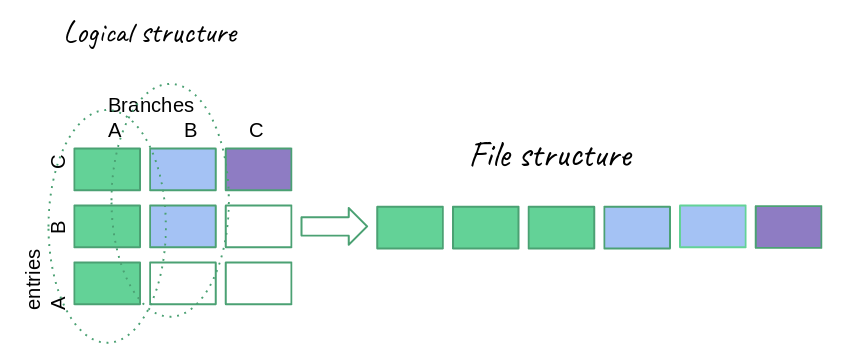
\includegraphics[width=0.8\linewidth]{rootio1.png}
\caption{ROOT I/O schema.  Data laid out logically into ``branches" and ``entries" (corresponding to columns and rows in a table) are serialized, column-wise, into buffers.  These buffers are then compressed and written into disk as part of a ROOT file.  The structure containing the buffers are referred to as `baskets'.}
\label{fig:rootio}
\end{figure}

Reading input in ROOT RIO subsystem consists primarily of decompression and deserialization operations. Compression and decompression are significant for ROOT I/O (see the Figure \ref{fig:rootio}) and are a ROOT core functionality.   The compressed baskets entries (green entries on the Figure \ref{fig:rootio} and a part of the logical structure of a ROOT file) present a number of advanced compression or decompression possibilities such as simultaneous read and decompression for the multiple physics events.

The available set of compression algorithms in ROOT are:
\begin{enumerate}
    \item \textit{ZLIB} - a LZ77 comprocessor with Huffman coding \cite{zlib}.
    \item \textit{LZMA} - one of LZ77 compressors, with significantly larger dictionary sizes compared to ZLIB and additional support for the repeatedly used match distances. Its output is encoded with a range encoder, using a complex model for probability prediction \cite{lzma}.
    \item \textit{Custom ROOT compression algorithm}.  This ZLIB-like compression algorithm, dating back to the 1990's, is used only for ROOT backward compatibility.
\end{enumerate}

% NOTE: Brian stopped here for the evening on 16 May

% TODO: cite previous work for LZ4?!? (Done)
For data compression, we have previously expanded the available set of compression algorithms in ROOT to cover a wider part of the performance phase space, specifically oriented to improving read speeds for analysis), shown on a Figure \ref{fig:compression}.
\begin{enumerate}
    \item \textit{LZ4} - a LZ77 compressor with a fixed, byte-oriented encoding and without Huffman coding pass \cite{lz4} \cite{brianzhe}.
    \item \textit{ZSTD} - a LZ77 algorithm supporting dictionaries, specialised by a large search window and entropy coding stage, using fast Finite State Entropy (tANS) or Huffman coding.\cite{zstd}
\end{enumerate}

In this article we would like to focus on comparison of compression algorithms, resulting in a new, analysis-oriented, default algorithm for ROOT in the latest development release, such as \textit{LZ4}, significant improvements of the compression speed of the prior default algorithm, such as \textit{ZLIB-CF}, and initial work on integrating a best-of-breed algorithm into ROOT, such as a \textit{ZSTD} compression algorithm.

\begin{figure}[h]
\centering
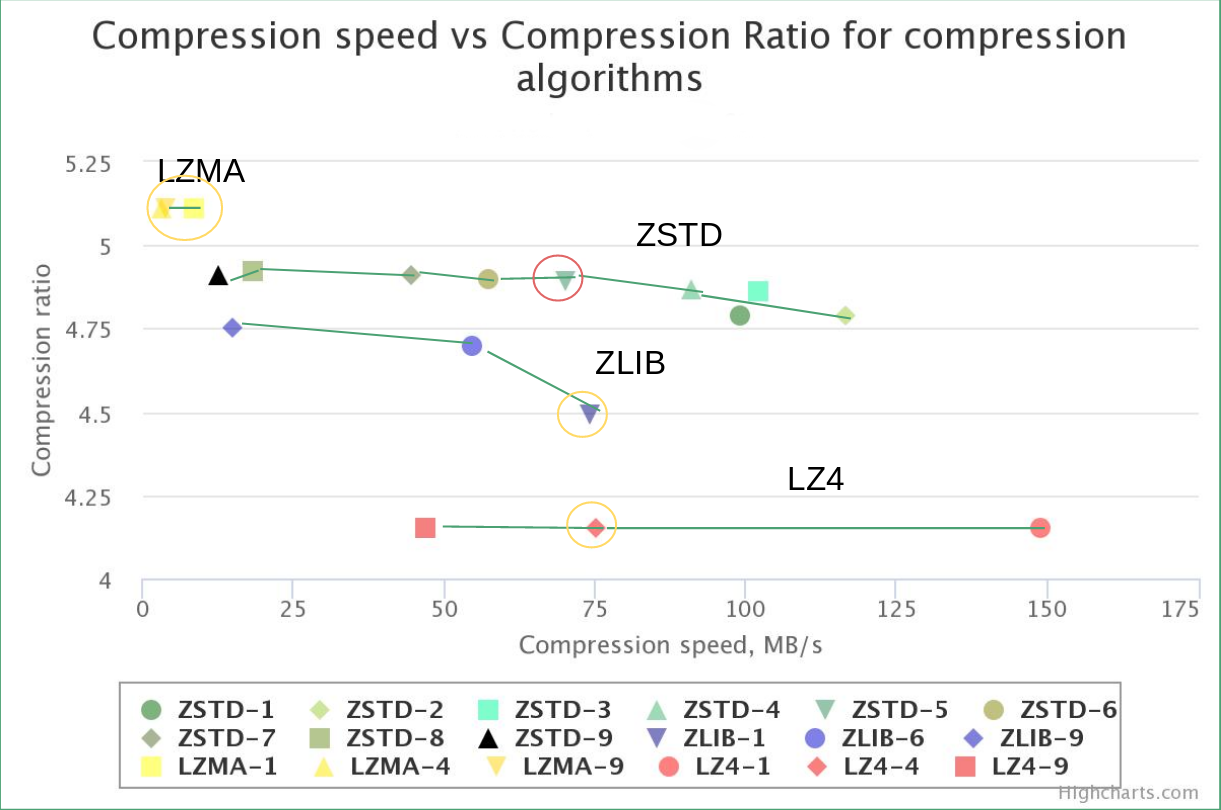
\includegraphics[width=0.8\linewidth]{compr.png}
\caption{ROOT compression algorithms comparisons for the  simplistic test case.}
\label{fig:compression}
\end{figure}

\begin{figure}[h]
\centering
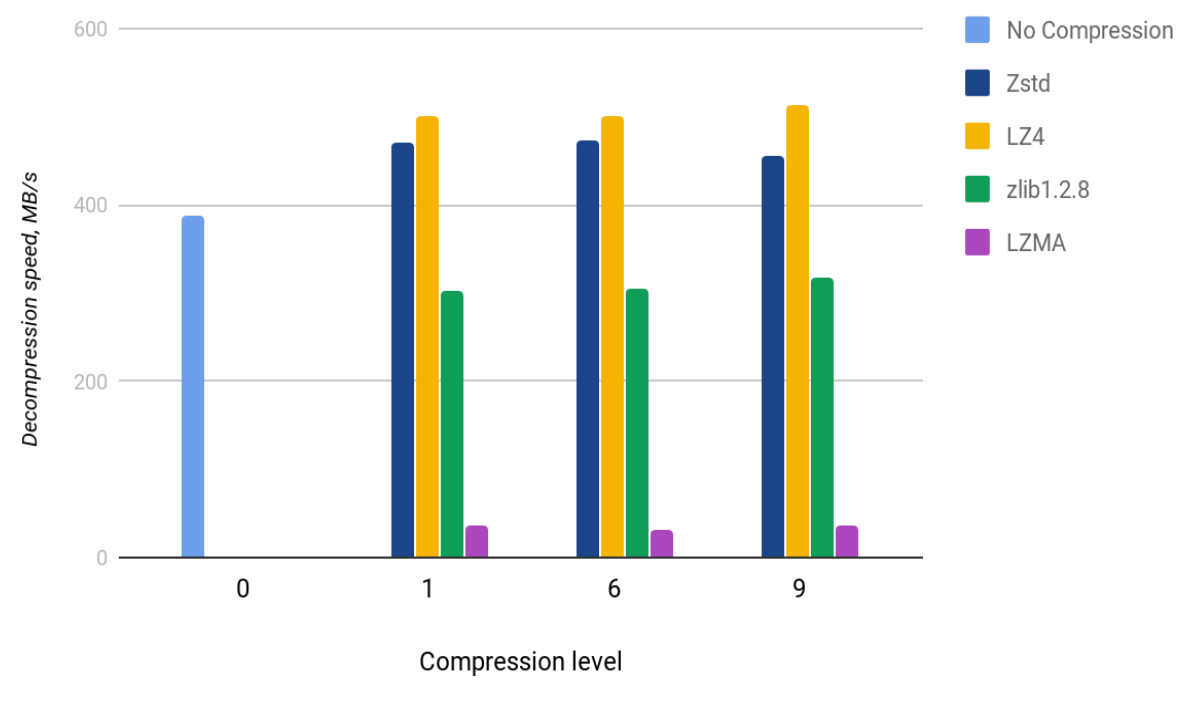
\includegraphics[width=0.9\linewidth]{acat11.png}
\caption{ROOT decompression algorithms comparisons for the simplistic test case.}
\label{fig:decompression}
\end{figure}

\subsection{Cloudflare Zlib}

This section describes a high performance modifications of \textit{Zlib} compression algorithm for Intel/ARMv8 processors and adopted in ROOT.

Classical \textit{deflate} compressed data format consists of a series of blocks, corresponding to successive blocks of input data. To be short, each block is compressed using a combination of the LZ77 algorithm and Huffman coding. Performance hotspots for \textit{Zlib} were identified as a \textit{adler32} checksum calculation and \textit{crc32} hash generation.
 
For systems supporting Intel SSE4.2 and AVX2, as well as NEON vector extentions in case of ARMv8, \textit{crc32} instructions are improving both hash performance and hash calculation quality. Both factors results in a the speed improvements of the hashing operations, and also improves the string-matching time for zlib. The same idea was used behind \textit{adler32} checksum generation widely used in zlib. Here SSE4.2 \textit{\_mm\_sad\_epu8()} can be used for byte sums  and for accumulation of the byte sums could be used SSE-style shuffle-adds.
 
 \textit{Zlib} uses a hash table for look up of the location of previous occurrences of a given string in the sliding history window. For the fast compression levels (1-5), \textit{improved Zlib} hashes all elements as quadruplets, having hash entry map to a match of four. This is a reason of reduction of a hash chain and better the quality factor for each match, while \textit{Zlib} provides only the opportunity to match to length of three (triplets). In addition, on the systems supporting Intel SSE4.2, AVX2 for Intel \& Neon for ARMv8, it was used \textit{crc32} instruction to provide a faster hash function.

\textit{Zlib} code base has a long history starting from 1995 and has previously been optimized for a set of old platforms and compilers. Excessive loop unrolling was one the efficient pattern in past, but not anymore needed for the modern processors, which are capable better scheduling of resources and executing instructions simultaneously. In \textit{Zlib} it is widely used in the \textit{adler32} and \textit{crc32} computations. In \textit{zlib-cf}, for the \textit{adler32} computation, it was reduced the unrolling factor from 16 to 8, and for \textit{crc32} computation, it was reduced from 8 to 4. 
 
 Finally for ROOT 6.18.00, we have contributed a set of patches for improving \textit{Zlib} performance as shown in Figure \ref{fig:cflaptop} and \ref{fig:cfneon}. The performance results provided on these figures were measured on an Intel®Core™ i7 Haswell laptop equipped with SSD and supporting Intel® SSE 4.2 and AVX2 instruction-set (Figure \ref{fig:cflaptop}) and Intel Haswell  Intel® Xeon® E5 v3 server.
 
 For the aarch64 platform was used ARCH64+CRC32 HiSilicon's Hi1612 processor (Taishan 2180) supporting Neon and hardware implementation of \textit{crc32} instructions (Figure \ref{fig:cfneon}) kindly provided by CERN Techlab. 

As a basis for developments was used sources of \textit{Cloudflare ZLIB} \cite{zlib-cf-sources} and its extended version \textit{CMS-ZLIB-CF} \cite{zlib-cf-cms} from CMS software stack. Both performance and compatibility with multiple platforms were further improved by DIANA-HEP. The new version is referred here and below as a “CF-ZLIB”. CF-ZLIB will be available in ROOT 6.18.00.

\begin{figure}[!ht]
\centering
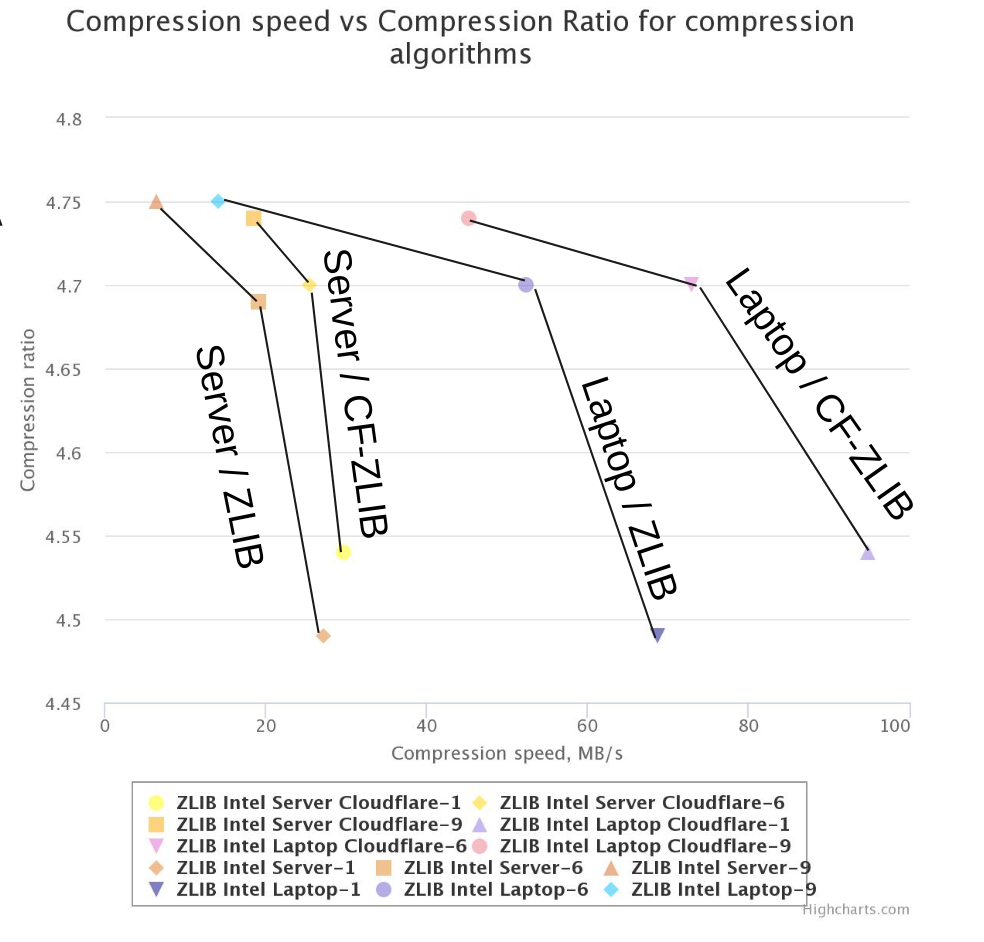
\includegraphics[width=0.7\linewidth]{acat21.png}
\caption{Compression speed improvements from the CF-ZLIB patch set on a laptop and server platform.  Note that, on the laptop platform, the speed of a high level of compression (CF-ZLIB-6) is now similar to the previous speed for the lowest compression level (ZLIB-1).}
\label{fig:cflaptop}
\end{figure}

\begin{figure}[!ht]
\centering
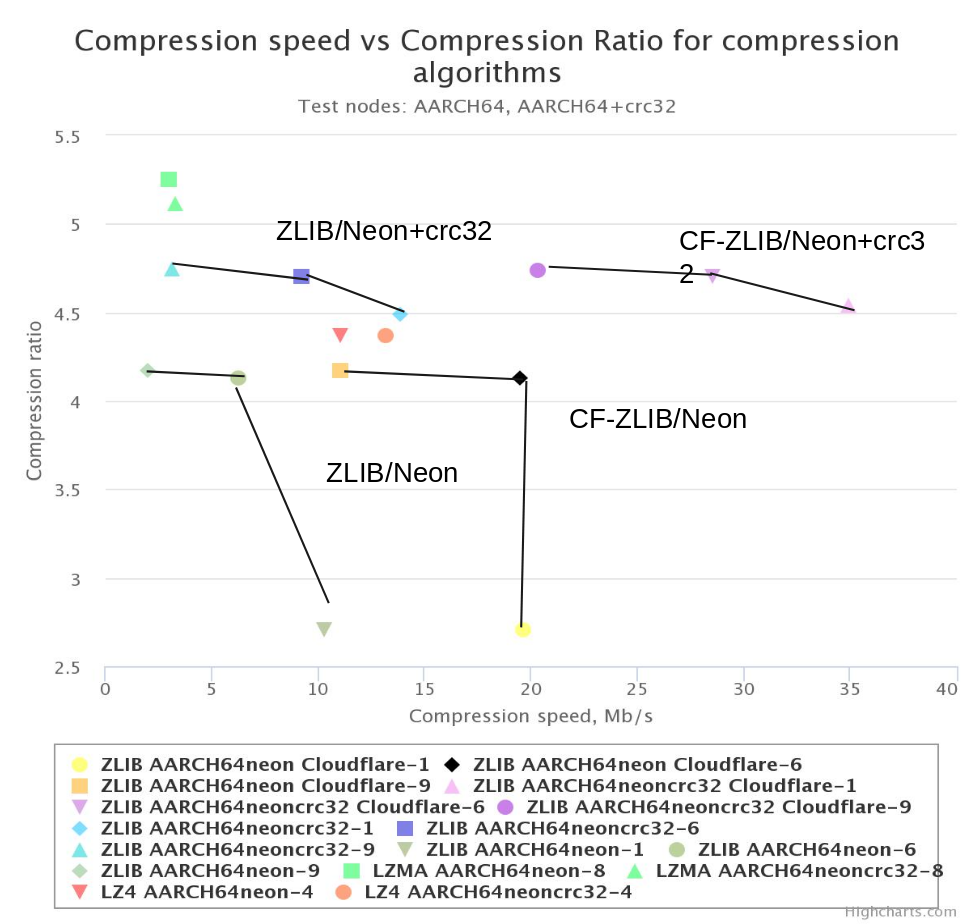
\includegraphics[width=0.7\linewidth]{acat31.png}
\caption{Compression speed improvements from the CF-ZLIB patch set for two different configurations: with hardware implementation of crc32 calculations and without.}
\label{fig:cfneon}
\end{figure}

\subsection{LZ4}

\textit{LZ4} is lossless compression algorithm, providing high competitive compression and decompression speed. One of the key features for it is an extremely fast decoder. It is a high speed compressor shipped together with \textit{LZ4} and called \textit{LZ4\_HC}, is available now in ROOT starting from ROOT version 6.14.00, trading customizable CPU time for compression ratio. The main difference with regular \textit{LZ4} is that the \textit{HC} version makes a full search, in contrast with the fast and not precise scan of the "regular" version \textit{LZ4}. It results in a compression ratio typically improved by 20\%. 

Significant improvements in \textit{LZ4} compression ratio inspired us to use \textit{LZ4\_HC} in ROOT. One of the disadvantages is an extra overhead that makes the compression speed impacted: the \textit{HC} version is actually slower than the \textit{LZ4-1}, a fastest setting for \textit{LZ4}, but still giving an advantage comparing to \textit{ZLIB-1} (see the comparison on Figure \ref{fig:compression}).

During tests of \textit{LZ4} as a default compression algorithm in ROOT was discovered a "corner case" for LZ4. One of the weak sides of \textit{LZ4} is a compression of small chunks of data, reported by user in case of TTree generated with variable-sized branches embed an “entry offset” array in their on-disk representation. Simplest solutions are usage of the compression pre-conditioners or dictionary compression (you can read more about it in the \textit{ZSTD} section). 

Pre-conditioners help to arrange bits of the values to compress sequences for primitive branches in ROOT TTree more efficiently. In case of pre-conditioners, the best algorithms that rearranges typed, binary data for improving compression ratio are:
\begin{enumerate}
    \item \textit{Shuffle} - integrated byte shuffle pre-conditioner (available in Blosc \cite{blosc})
    \item \textit{BitShuffle} - integrated bit shuffle pre-conditioner (available in Blosc \cite{blosc})
\end{enumerate}

Preliminary results is showing the promising results(Figure \ref{fig:bitshuffle}). It is a promising result that shows that \textit{LZ4} can outperform \textit{ZLIB} by better compression ratio, while compression time should be still optimized.
\begin{figure}
\centering
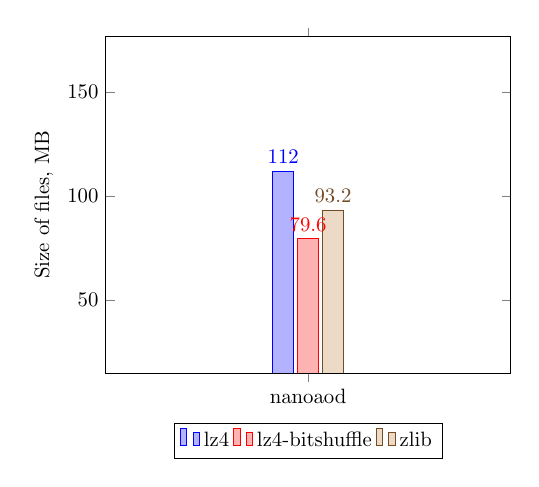
\begin{tikzpicture}[scale=0.75]
\begin{axis}[
    ybar,
    enlargelimits=1.99,
   % width=0.99\textwidth,
    legend style={at={(0.5,-0.15)},
      anchor=north,legend columns=-1},
    ylabel={Size of files, MB},
    symbolic x coords={nanoaod},
    xtick=data,
    nodes near coords,
    nodes near coords align={vertical},
    ]
\addplot coordinates {(nanoaod,112)};
\addplot coordinates {(nanoaod,79.6)};
\addplot coordinates {(nanoaod,93.2)};
\legend{lz4,lz4-bitshuffle,zlib}
\end{axis}
\end{tikzpicture}
\caption{Bitshuffle filter used for LZ4 compression of NanoAOD file in ROOT.} \label{fig:bitshuffle}
\end{figure}

%In case of usage of the dictionaries, sadly \textit{LZ4} doesn't support dictionary generation. Then dictionary can be created by using \textit{ZSTD} \cite{zstd}: \textit{zstd --train} on a set of samples. Interesting fact is that generated output after \textit{ZSTD} is compatible with \textit{LZ4}. One of the limitations are that dictionary size which should be less or equal then 64 KB, since \textit{LZ4} will not be able to use more content anyway. Tests shows that the speed could be faster than in case of \textit{Zlib}, by an order of magnitude. Other pleasant optimisation could be achieved simple enable aggressive compilation flags optimisation and may influence the result in less or equal 20 \% improvement.

\subsection{ZSTD}

The initial promise of \textit{Zstandard} \cite{zstd} \cite{zstd-facebook} was that it would allow users or software frameworks to replace their existing data compression implementation (e.g., for example for the ROOT, it is \textit{Zlib} or \textit{LZ4} depending on ROOT version) with improved compression ratio, compression speed, and decompression speed. A new interesting features offered by \textit{ZSTD} and considered to be competitive comparing to other algorithms, are bigger block size, compression dictionary support and many others.

The block size for \textit{ZSTD} is now 256 KB, which it is eight times larger than the size of the \textit{Zlib} window. Additional effort by \textit{ZSTD} developers was put into an optimisation of the data transformations that were designed to outperform the \textit{Zlib} compression.  With search history limited to 32 KB, profiling of \textit{Zlib} showed a lot of redundant operations that could be better optimized. Meanwhile \textit{ZSTD} is able to analyze larger history and  achieved reduction for the number of transformation stages allows to save in CPU capacity, memory, and latency. This improvements could be very interesting for the data and storage management for the software frameworks, in terms of Run 3 requirements provided by \textit{LHC} experiments \cite{zstd-facebook}. 

The top level feature of \textit{ZSTD} is a dictionary generation. A dictionary makes it possible for the compression algorithm's compressor to start from a meaningful state instead of an empty one. It makes compression much more effective, even when compressing a small amount of data, such as a few hundred bytes. The dictionary is generated by analyzing sample data, presuming that the rest of the data to compress will be a similar. As a part of distribution process, dictionary could be provided along as a part of ROOT file.

All together, these and many others features make \textit{ZSTD} a powerful and flexible compressor engine that was developed and  widely used by top industry companies as Facebook. \textit{ZSTD} can outperform \textit{Zlib} and provides the benefits that could be useful in multiple HEP scenarios that were traditionally difficult for "classical" compressors.

Preliminary investigation results for \textit{ZSTD} is shown at the Figure \ref{fig:compression} and Figure \ref{fig:decompression}. \textit{ZSTD} is planned to available in ROOT 6.20.00.

\section{Results}
As part of the DIANA-HEP initiative to improve ROOT-based analysis, we have continued work in comparing compression algorithms \cite{brianzhe}. In the scope of this article, we included a detailed overview of pro and cons of main existing compression algorithms such as LZ4, ZSTD, ZLIB and ZLIB-CF. Results could be used for evaluation of ROOT I/O and in particularly, its compression and decompression functionality. 

Future work items include work on re-enabling \textit{LZ4} as a default ROOT compression algorithm, work on improvement of I/O interfaces for easier switching between compression algorithms and further work on optimization of compression algorithms in ROOT (using of compression dictionaries and etc.). ROOT I/O performance could be tracked using the automatized performance benchmarking suite for ROOT \cite{rootbench}.

\section{Acknowledgments}

This work has been supported by U.S. National Science Foundation grant ACI-1450323.

\section{References}

\begin{thebibliography}{10}
\bibitem{zlib-cf}
Kukunas, J. T., Gopal, V., Guilford, J., Gulley, S., van de Ven, A., \& Feghali, W. (2014). High performance ZLIB compression on Intel® architecture processors. White paper, April.

\bibitem{zlib-cf-sources}
GitHub. 2019. GitHub - cloudflare/zlib: Cloudflare fork of zlib with massive performance improvements. [ONLINE] Available at: https://github.com/cloudflare/zlib. [Accessed 11 May 2019]. 

\bibitem{zlib-cf-cms}
GitHub. 2019. GitHub - cms-externals/zlib: A massively spiffy yet delicately unobtrusive compression library.. [ONLINE] Available at: https://github.com/cms-externals/zlib.git. [Accessed 11 May 2019]. 

\bibitem{zstd}
Collet, Y. and M. Kucherawy, Ed., "Zstandard Compression and the application/zstd Media Type", RFC 8478, DOI 10.17487/RFC8478, October 2018, <https://www.rfc-editor.org/info/rfc8478>.

\bibitem{zstd-facebook} 
Facebook Code. 2019. Zstandard: How Facebook increased compression speed - Facebook Code. [ONLINE] Available at: https://code.fb.com/core-data/zstandard/. [Accessed 11 May 2019]. 

\bibitem{zlib}
Deutsch, P. and J-L. Gailly, "ZLIB Compressed Data Format Specification version 3.3", RFC 1950, DOI 10.17487/RFC1950, May 1996, <https://www.rfc-editor.org/info/rfc1950>.

\bibitem{lz4}
GitHub. (2019). lz4/lz4. [online] Available at: https://github.com/lz4/lz4/blob/master/doc/
lz4\_Frame\_format.md [Accessed 11 May 2019].

\bibitem{lzma}
Tukaani.org. (2019). XZ Utils. [online] Available at: https://tukaani.org/xz/ [Accessed 11 May 2019].

\bibitem{brianzhe}
Z. Zhang and B. Bockelman. "Exploring compression techniques for ROOT IO" 2017 J. Phys.: Conf. Ser.898 072043

\bibitem{blosc}
GitHub. 2019. GitHub - Blosc/c-blosc: A blocking, shuffling and loss-less compression library that can be faster than `memcpy()`.. [ONLINE] Available at: https://github.com/Blosc/c-blosc. [Accessed 14 May 2019]. 

\bibitem{rootbench}
Oksana Shadura, Vassil Vassilev and Brian Paul Bockelman, \textit{Optimizing Frameworks Performance Using C++ Modules Aware ROOT}, CoRR, http://arxiv.org/abs/1812.03149

\end{thebibliography}

\end{document}

